\section{Design of Cascade Controller}
In this section, controllers for the two cascade loops are to be designed. First the inner loop is designed and afterwards the outer loop is designed. These will afterwards be verified in a later section. 

\subsection{Inner Loop}
In this section the inner loop controller is designed. The inner loop has the purpose of controlling the motors and wheels model and ensure that the effect of noise and uncertainties in the system are diminished, resulting in better performance for the balancing segway.\newpage
The transfer function for the motors and wheels is:
%that the input for the outer loop, the inverted pendulum model, is 1, as this will eliminate noise and ensure a more efficient cascade controller. This will result in a more stable balancing segway. The motors and wheels model is the following expression.
\begin{equation}
G_2(s)=\frac{17.72}{s+9.799} = \frac{1.81}{0.10s + 1}
\end{equation}
\begin{where}
\va{$G_2(s)$}{is the plant of the inner loop}{1}
\end{where}

The motors and wheels model is a first order system with a pole in -9.799. This means it is a type 0 system, as it does not have any poles in zero. This reveals some characteristics of the system. One of these is the presence of a steady-state error in its step response \citep[p. 211]{sou:Feedback}. This can only be fully eliminated if an integrator is implemented, as this yields a type 1 system. It is however chosen not to do this, but instead only implement a gain as this is assumed to reduce the steady-state error adequately and allows for a simpler controller design. A P-controller is therefore designed for the inner loop. A P-controller has the form as seen below:
\begin{equation}
D_2(s)=k_{p2}
\end{equation}
\begin{where}
\va{$D_2(s)$}{is the controller for the inner loop}{1}\\
\va{$k_{p2}$}{is the proportional gain}{1}
\end{where}

To design a P-controller it is necessary to look into how fast the system is sampled as this, together with saturation, sets an upper limitation for how much gain the system can handle. However, in the design of this controller, the saturation is disregarded as it is assumed that the influence is negligible. The motors' encoders sample with a frequency of 1 kHz. This is also the frequency of the inner loop. It is preferable, by rule of thumb, to have a system bandwidth that is more than 25 times smaller than the angular sampling frequency \citep[p. 613]{sou:Feedback}. It is however chosen to design with a factor of 10. Note that the sampling frequency is converted from hertz to radians per seconds, and thus the bandwidth is found as:

\begin{equation}
\omega_{BW} = 2\pi\cdot \frac{f_s}{10}= 2\pi\cdot\frac{1000}{10}= 628.32 \label{eq:motorbandwidth}
\end{equation}
\begin{where}
\va{$\omega_{BW}$}{is the bandwidth of the inner loop}{rad/s}
\va{$f_s$}{is the sampling frequency of the inner loop}{Hz}
\end{where}

From \autoref{eq:motorbandwidth} the bandwidth of the plant in the inner loop is found to be 628.32 rad/s. By examining the bode plots of the plant without a controller, the plant's gain can be determined.\vspace{-1 cm}
\begin{figure}[H]
\centering
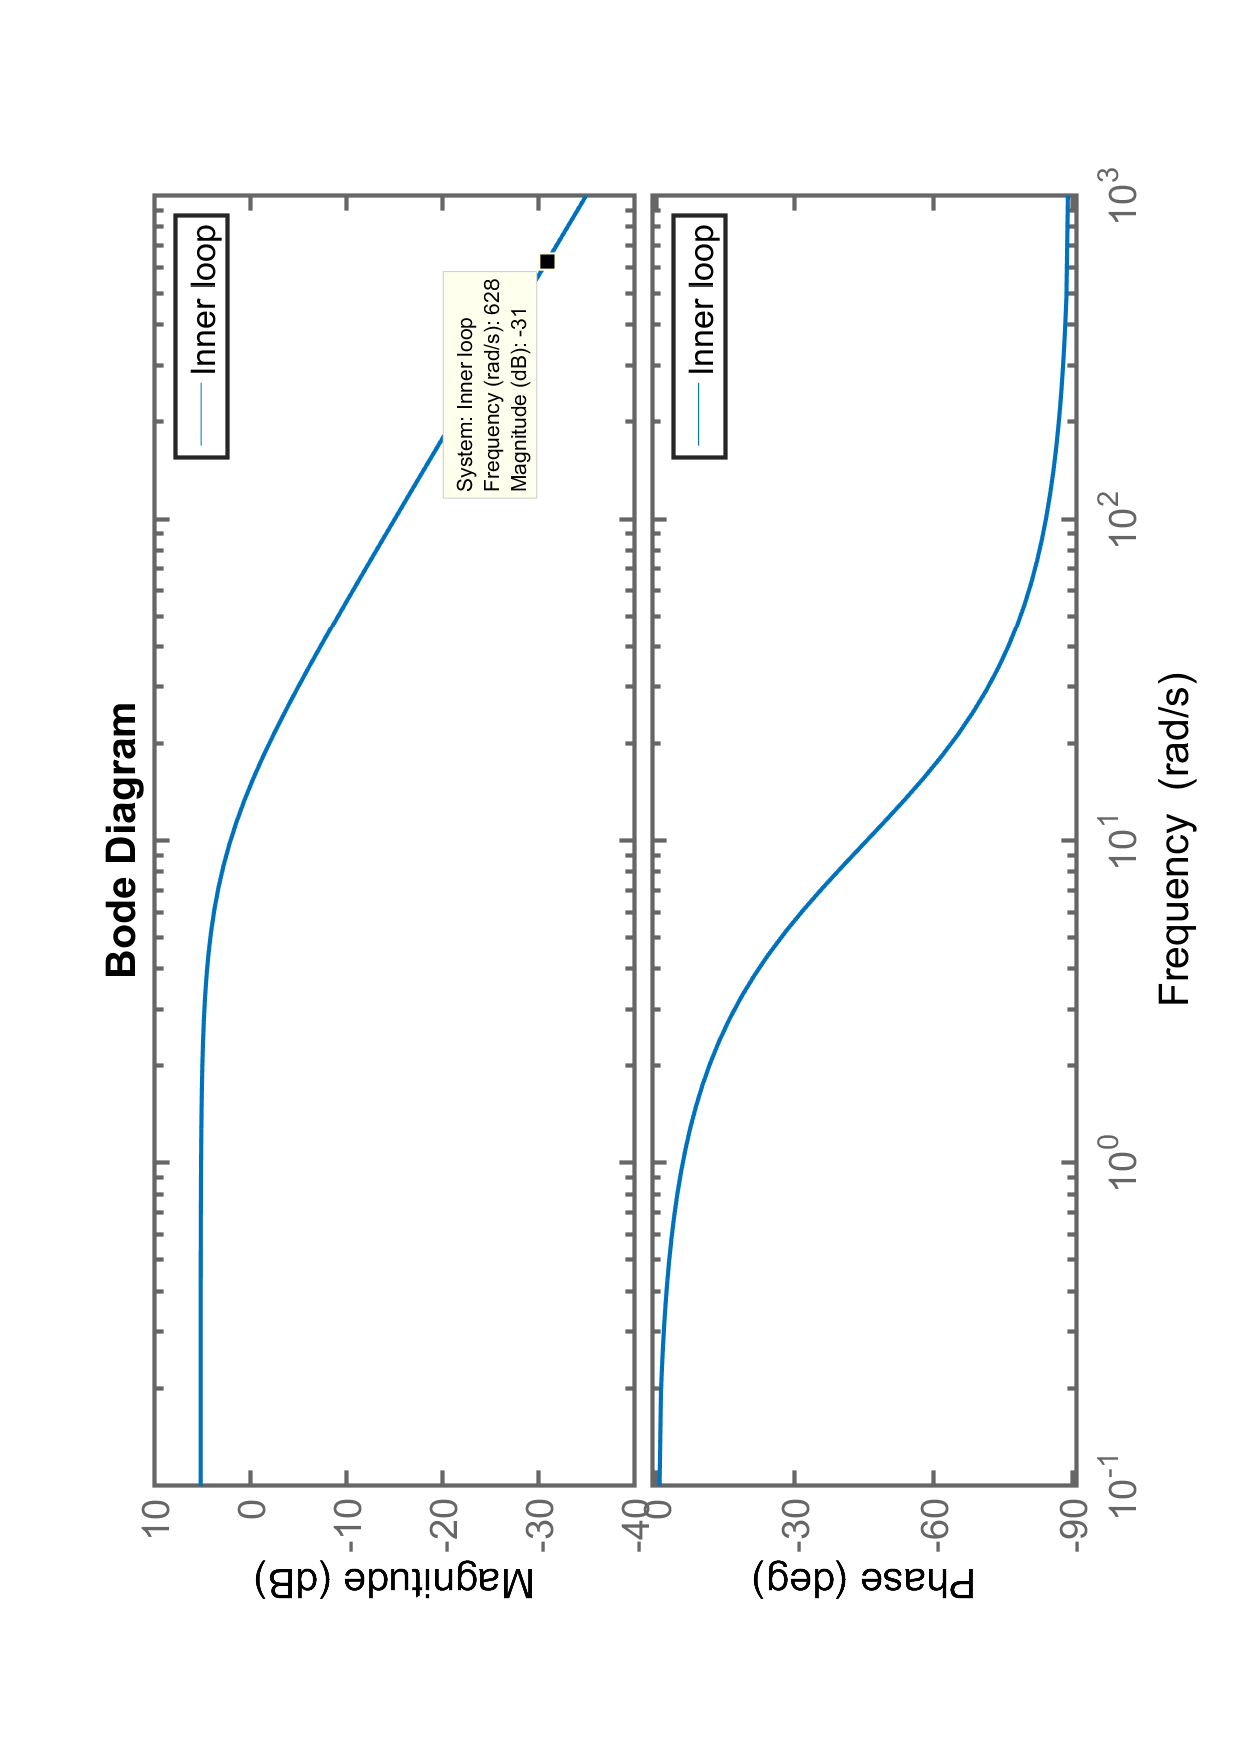
\includegraphics[height = \textwidth, angle = -90]{bodemotorplant.pdf}
\caption{Open loop bode plots of motors and wheels model, where the controller has a gain of 1. The approximate bandwidth, 628 rad/s, is marked.}
\label{fig:bodemotorplant}
\end{figure}
\vspace{-0.7 cm}
From \autoref{fig:bodemotorplant} it can be seen that the magnitude is approximately -31 dB. To obtain a magnitude of -3 dB, the graph shall be lifted 28 dB. The scalar gain can be found as follows:
\begin{equation}
k_{p2}=10^\frac{28}{20}= 25.11 \label{eq:dbscalar}
\end{equation}
The P-controller has now been designed and will in the following section be verified.
\subsection{Verification of Inner Loop Controller}
The gain for the inner loop controller shall be 25.11 according to \autoref{eq:dbscalar}. The transfer function of the closed loop can be expressed as shown in \autoref{eq:clmotor} where $H_2(s)$ is 1, due to no gain in the sensor block.
\begin{align}
\frac{Y_2(s)}{R_2(s)}=\frac{D_2(s)\cdot G_2(s)}{1+D_2(s)\cdot G_2(s)\cdot H_2(s)}
= \frac{25.11\frac{17.72}{s+9.799}}{1+25.11\frac{17.72}{s+9.799}} \label{eq:clmotor}
\end{align}
\begin{where}
\va{$Y_2(s)$}{is the output of the inner loop}{1}\\
\va{$R_2(s)$}{is the reference to the inner loop}{1}\\
\va{$H_2(s)$}{is the sensor block in the inner loop}{1}
\end{where}

\begin{figure}[H]
\centering
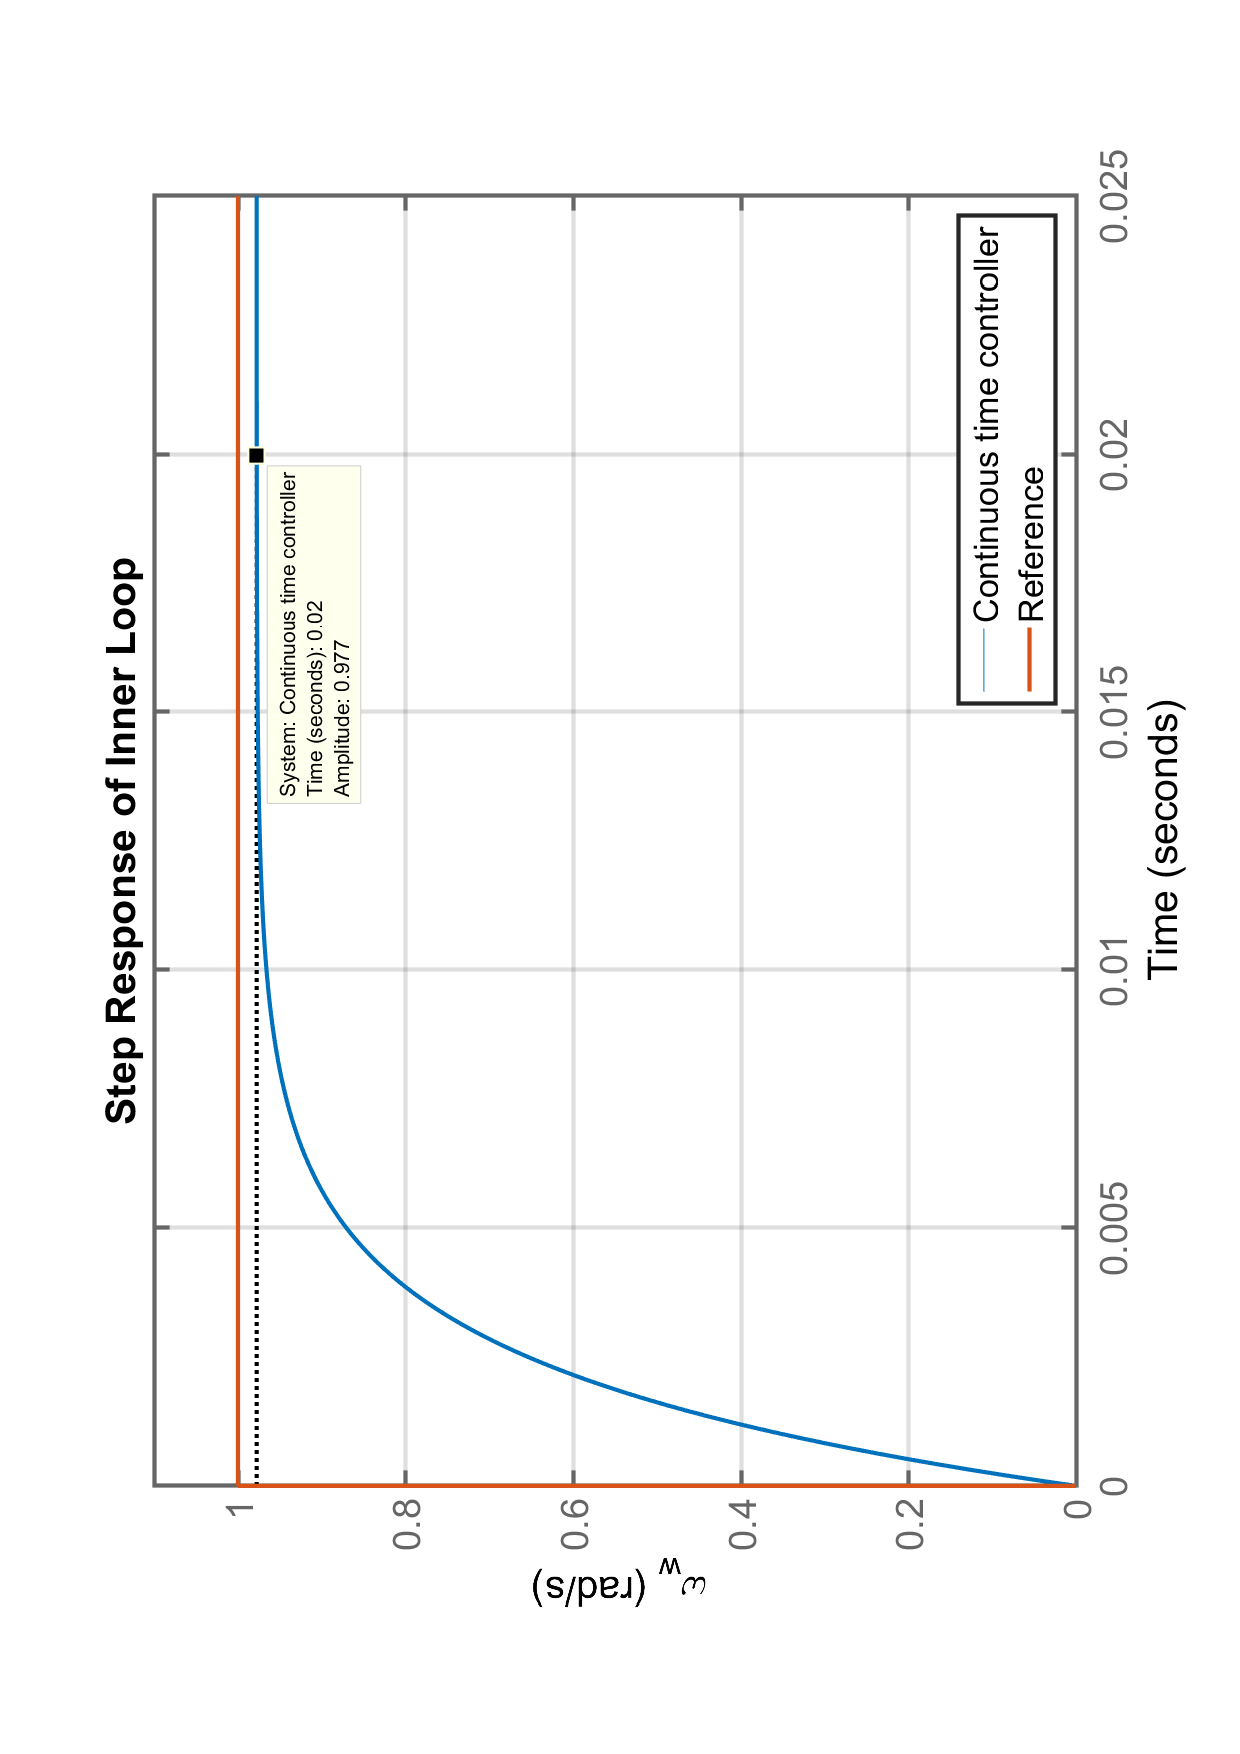
\includegraphics[height = \textwidth, angle = -90]{stepmotor25.pdf}
\caption{Simulation of the step response for inner loop with the designed continuous time P-controller.}
\label{fig:stepmotorcontroller}
\end{figure}

From \autoref{fig:stepmotorcontroller} it can be seen, that the steady-state error is 2.2\% which is deemed small enough that effect of this error on the full segway system is negligible. When looking at the characteristic equation, which is the main denominator in the closed loop transfer function, it can be seen that the gain changes the pole placement. The pole is moved far out in the left half plane (LHP). This increases the speed of the inner loop's dynamics, which can be seen in \autoref{fig:stepmotorcontroller}, where the step response settles within 0.02 seconds. 
%This results in the outer loop's input being 1, which is desired.\\ 

The closed loop transfer function is now discretized using MATLAB. The method used is the bilinear transformation, which is further described in \autoref{sec:bilinear}. This yields:
\begin{equation}
\frac{Y_2(z)}{R_2(z)} = \frac{0.2151 z^2 + 0.002119 z - 0.213}{ 1.215 z^2 - 1.978 z + 0.7674}
\end{equation}

This is compared to the continuous time controller which can be seen in \autoref{fig:sysStep1}. 

\begin{figure}[H]
\centering
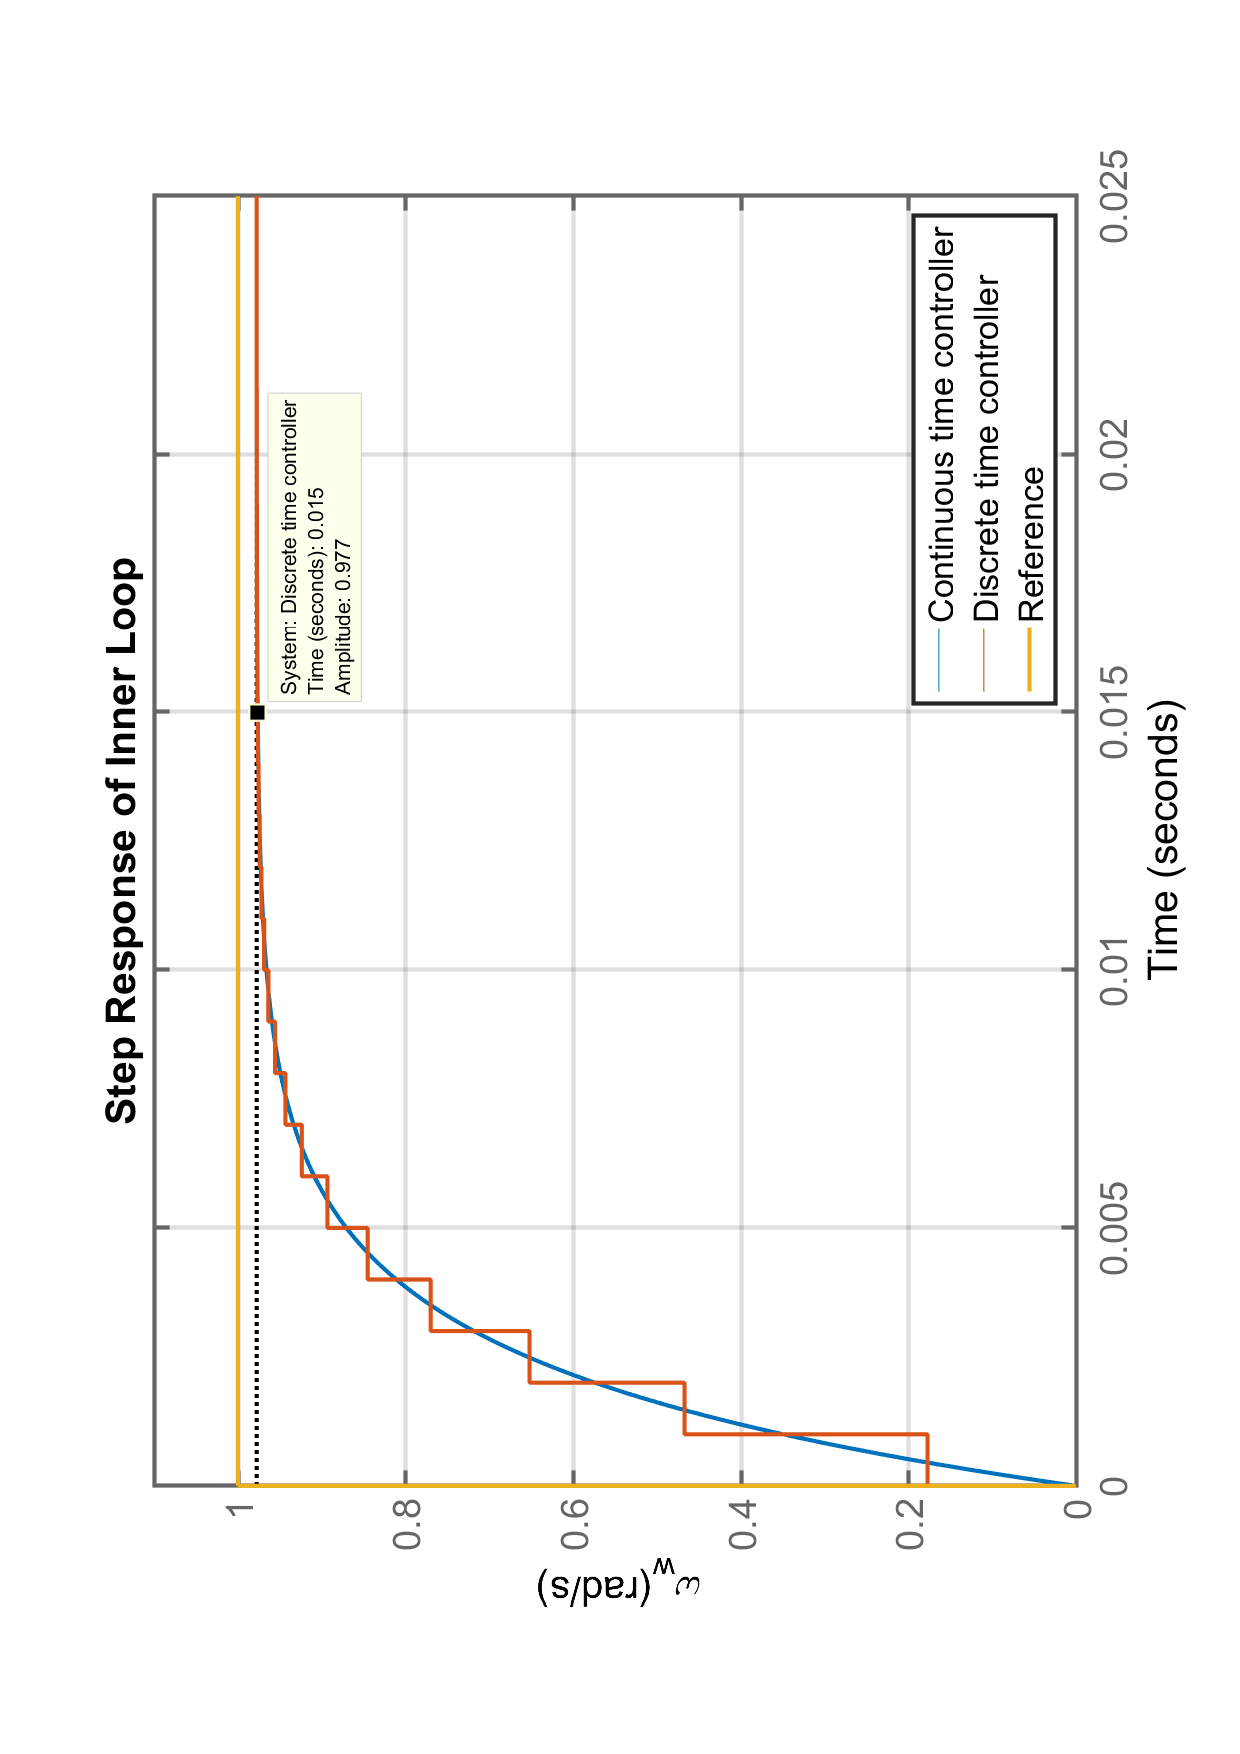
\includegraphics[height =\textwidth ,angle = -90]{sysStep1.pdf}
\caption{Simulation of the step response of continuous and discrete time inner loop controller.}
\label{fig:sysStep1}
\end{figure}

From \autoref{fig:sysStep1} it can be seen that the discrete controller matches the continuous controller and the P-controller with a gain of 25.11 for the inner loop is hereby derived. It can further be seen, that at 15 ms the velocity has almost reached its steady-state value, which means that if 15 ms is chosen as sampling time for the outer loop, the inner loop can be seen as 1 in this regard.

The outer loop will be designed in the following section. These two loops forms the cascade controller for the full system.
%\begin{figure}[H]
%\centering
%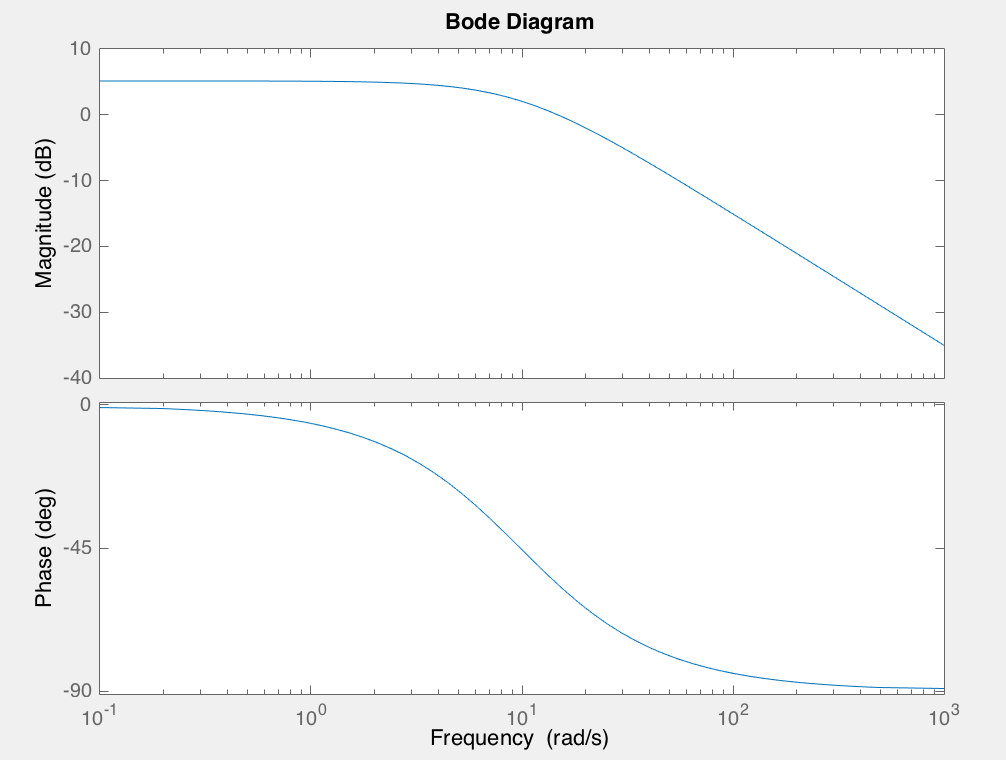
\includegraphics[scale=0.75]{figures/bodemotor.PNG}
%\caption{Bodeplot of the motors and wheels model.\label{fig:bode:motor:A}} 
%\end{figure}
%Standard method, bodeplot\\
%As the model is stable it is possible to design the controller from the bodeplot in \autoref{fig:bode:motor:A}. 
%As the motors and wheels model is the inner loop, it has to be fairly faster than the outer loop, as it then can be persived as one, as it is assumed that it will achieve steady state within the time before the outer loop is recieving it as input. A P-controller is therefore suitable for this purpose. A P-controller is just a gain multiplied with the error signal. From the bodeplot, \autoref{fig:bode:motor:A}, a $K_p$ constant of 10 is derieved. 
%To be continued! .... 
%\begin{figure}[H]
%\centering
%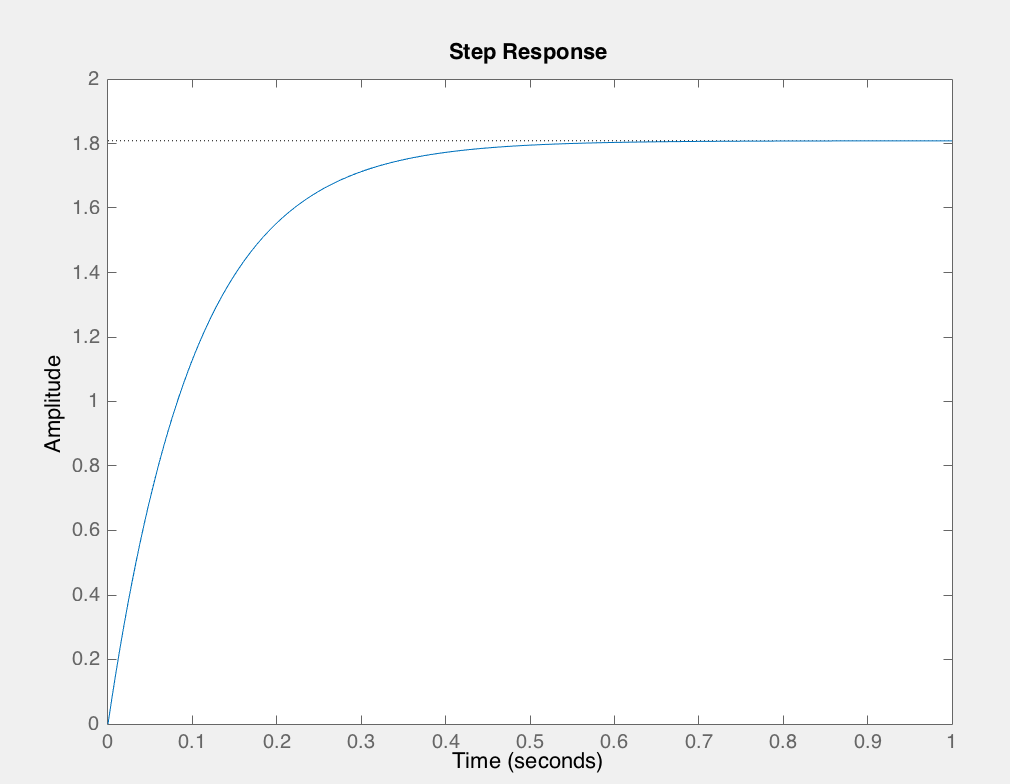
\includegraphics[scale=0.75]{figures/stepmoter.PNG}
%\caption{Stepresponse of the motor without controller.} 
%\end{figure}
%step response (assosiated input)
\subsection{Outer Loop}
In this section a controller is designed for the inverted pendulum, who's transfer function can be seen in \autoref{eq:OuterLoopPlant}. It can be seen that there is a pole in the right half plane (RHP), meaning that the system is unstable. The controller is therefore designed with the primary purpose of stabilizing the system. Additional requirements that are not met by this controller can be met by the use of compensators, such as lag or lead-lag compensators. \newpage
The transfer function of the inverted pendulum is the following:
\begin{equation}
\frac{\Theta_p(s)}{\Omega_w(s)}=\frac{0.2367\cdot s}{s^2 - 21.92} = \frac{0.2367 \cdot s}{(s + 4.682)(s - 4.682)}\label{eq:OuterLoopPlant}
\end{equation}
%The main concern for the outer loop controller is to move the plant's RHP pole, so that there will only be LHP poles in the closed loop. 
The first step is to move the pole that makes the system unstable to the left half plane (LHP), by adding a zero in the LHP to the left of the leftmost plant pole \citep[p. 273]{sou:Feedback}. The second step is to add a gain, which actually moves the poles. This can be implemented with a PD-controller in the form of:
\begin{equation}
D_1(s) = (s - k_z)k_{p1}
\end{equation}
\begin{where}
\va{$k_z$}{is the location of the zero}{1}\\
\va{$k_{p1}$}{is the proportional factor}{1}\\
\end{where} 
\vspace{-0.5 cm}

With this controller type, there will be two zeros and two poles in the open loop. Increasing the $k_{p1}$ value will cause each pole to move closer to a zero. Leading to that the RHP pole will end in the zero in origin and the LHP pole will end in the LHP zero \citep[p. 268]{sou:Feedback}. This makes it impossible to move the RHP pole into the LHP, as it will stop in the origin, due to the zero there. Therefore this zero has to be cancelled. This is done through pole-zero cancellation, by adding an integrator to the controller. This yields the following PID-controller:
\begin{equation}
D_1(s) = \frac{(s - k_z)k_{p1}}{s}
\end{equation}
The zero has to be placed in the LHP to the left of the leftmost plant pole, as this causes the root locus shown in \autoref{fig:locus1}. The zero is placed in $-10$ to give a margin for errors in the model. Thus $k_z = -10$.
\vspace{-1 cm}
\begin{figure}[H]
\centering
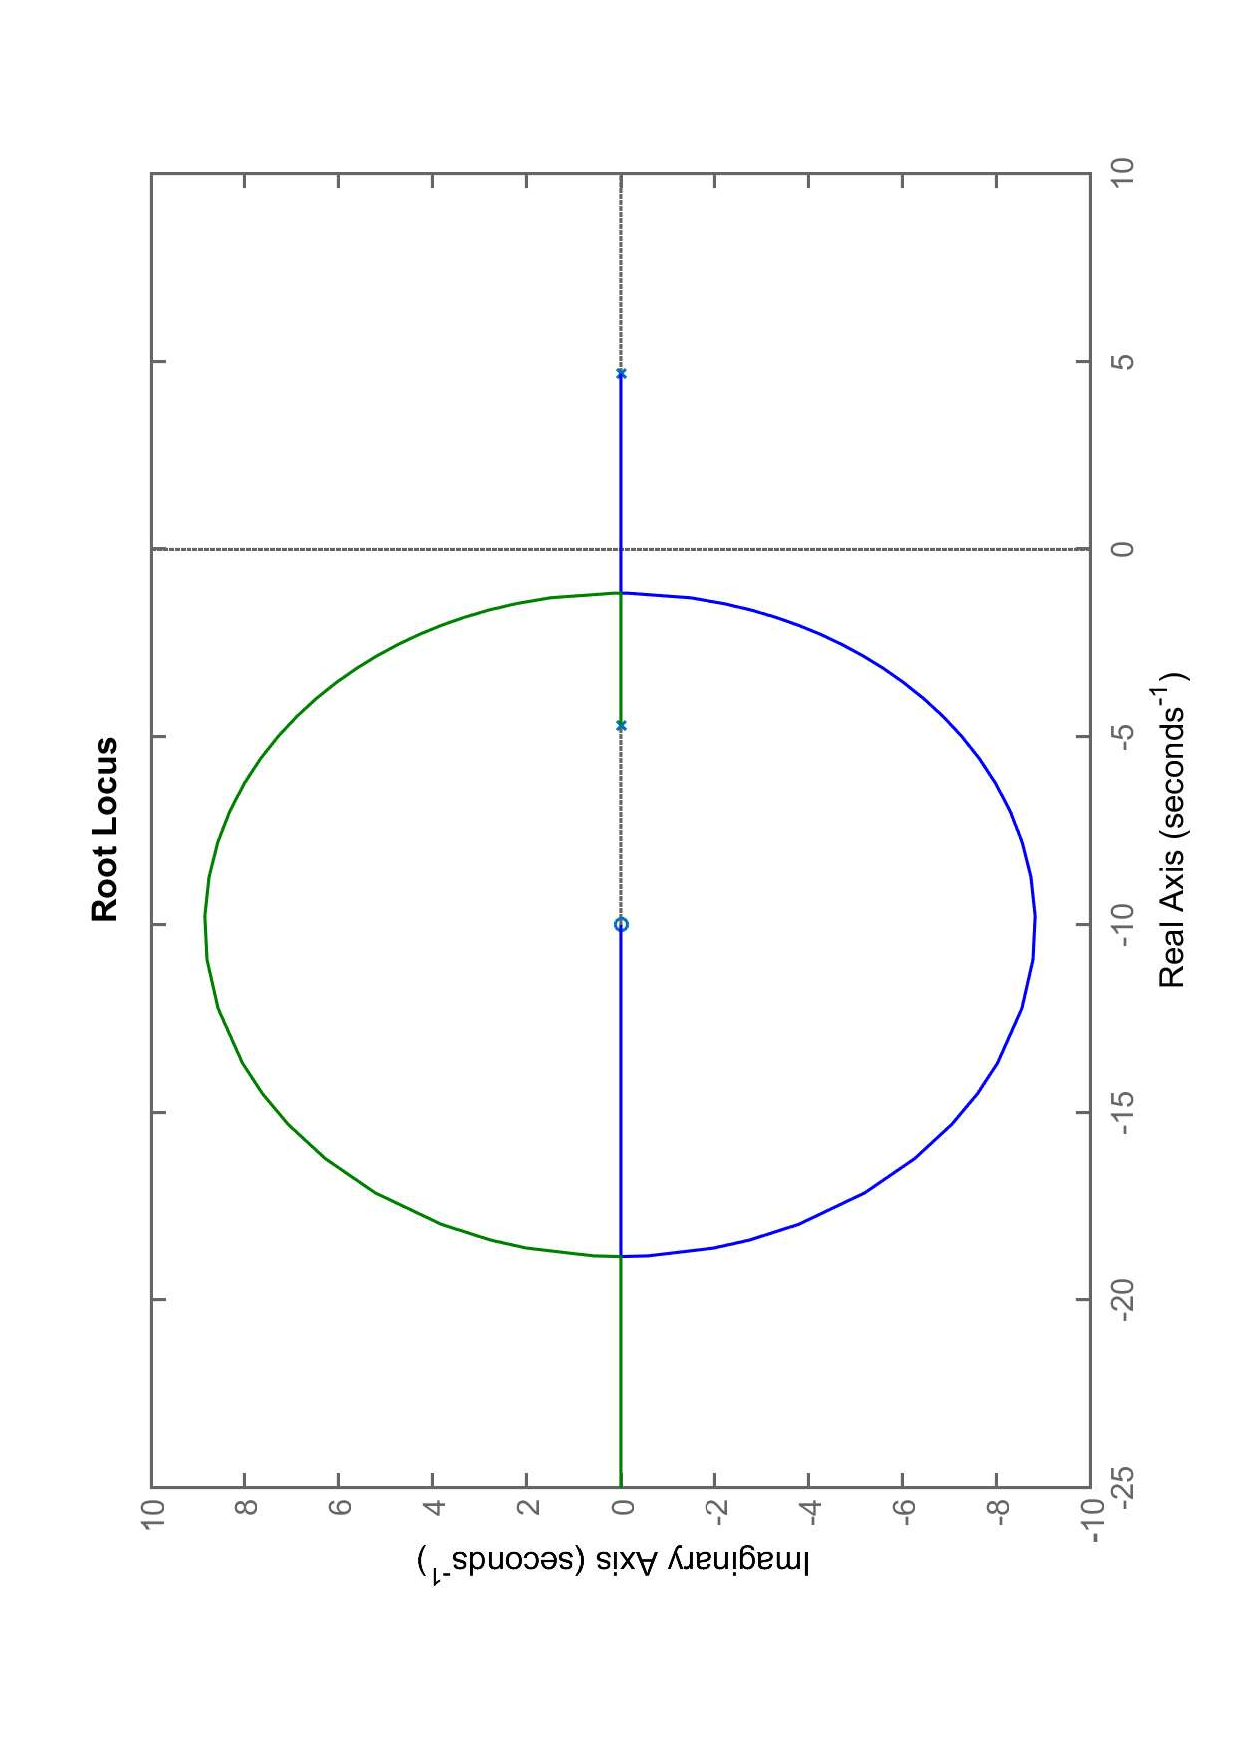
\includegraphics[height=0.90\textwidth,angle = -90]{locus1.pdf}
\vspace{-0.5 cm}
\caption{The root locus of the system, where a zero has been inserted in -10 and an integrator has cancelled the zero in origin.}
\label{fig:locus1}
\end{figure}
The task now is to determine the $k_{p1}$ factor. This is done through consideration of the requirements. The requirement for overshoot, MP, is that it has to be within 10\%. This yields a damping, $\zeta$, of $0.8$, as the plant is a second order system. This value is calculated with \autoref{eq:MPcal} \citep[p. 153]{sou:Feedback}.
\begin{equation}
MP = e^\frac{-\pi \cdot \zeta}{\sqrt{1 - \zeta^2}} \label{eq:MPcal}
\end{equation}
The bandwidth, $\omega_{BW}$, is now calculated based on the sampling frequency, $f_s$, in the same manner as done for the inner loop:
\begin{equation}
\omega_{BW} = 2 \cdot \pi \frac{f_s}{10} = 2 \cdot \pi \frac{1}{T_s \cdot 10} = 2 \cdot \pi \frac{1}{15 \cdot 10^{-3} \cdot 10} = 41.888
\end{equation}
\begin{where}
\va{$\omega_{BW}$}{is the bandwidth of the system}{$\frac{rad}{s}$}\\
\va{$f_s$}{is the sampling frequency}{$\frac{1}{s}$}\\
\va{$T_s$}{is the sampling time}{$s$}\\
\end{where}
The natural frequency can be calculated as shown in \autoref{eq:omegBWtoomegn} \citep{sou:control_slide7}:
\begin{equation}
\omega_n \approx \frac{\omega_{BW}}{1.4} = \frac{41.888}{1.4} = 29.92\label{eq:omegBWtoomegn}
\end{equation}
\begin{where}
\va{$\omega_n$}{is the natural frequency}{$\frac{rad}{s}$}\\
\end{where}

Thus the highest allowable $\omega_n$ is $29.92 \frac{rad}{s}$, which yields an approximate rise time, $t_r$, as calculated in \autoref{eq:riseTime} \citep[p. 152]{sou:Feedback}.

\begin{equation}\label{eq:riseTime}
t_r \approx \frac{1.8}{\omega_n} = \frac{1.8}{29.92} = 0.060
\end{equation}
\begin{where}
\va{$t_r$}{is the rise time of the step response}{$s$}\\
\end{where}

This rise time is considerably less than the 1 second from the requirements, thus the $\omega_n$ leads to this requirement being fulfilled. The fast rise time may however lead to saturation problems, as a fast rise time requires a high control gain, leading to a high controller output, making saturation more likely. This will be dealt with through tuning.

The open loop is now plotted as a root locus, and the damping, $\zeta$ and natural frequency, $\omega_n$, are inserted as boundaries. The white area fulfills the requirements and thus the poles should be placed here. The $k_{p1}$ value is chosen to be 160, yielding the pole locations shown in \autoref{fig:locus2}. The poles are placed on the real axis close to the break-in-point, as a high gain yields a low steady-state error and overshoot.
\vspace{-1 cm}
\begin{figure}[H]
\centering
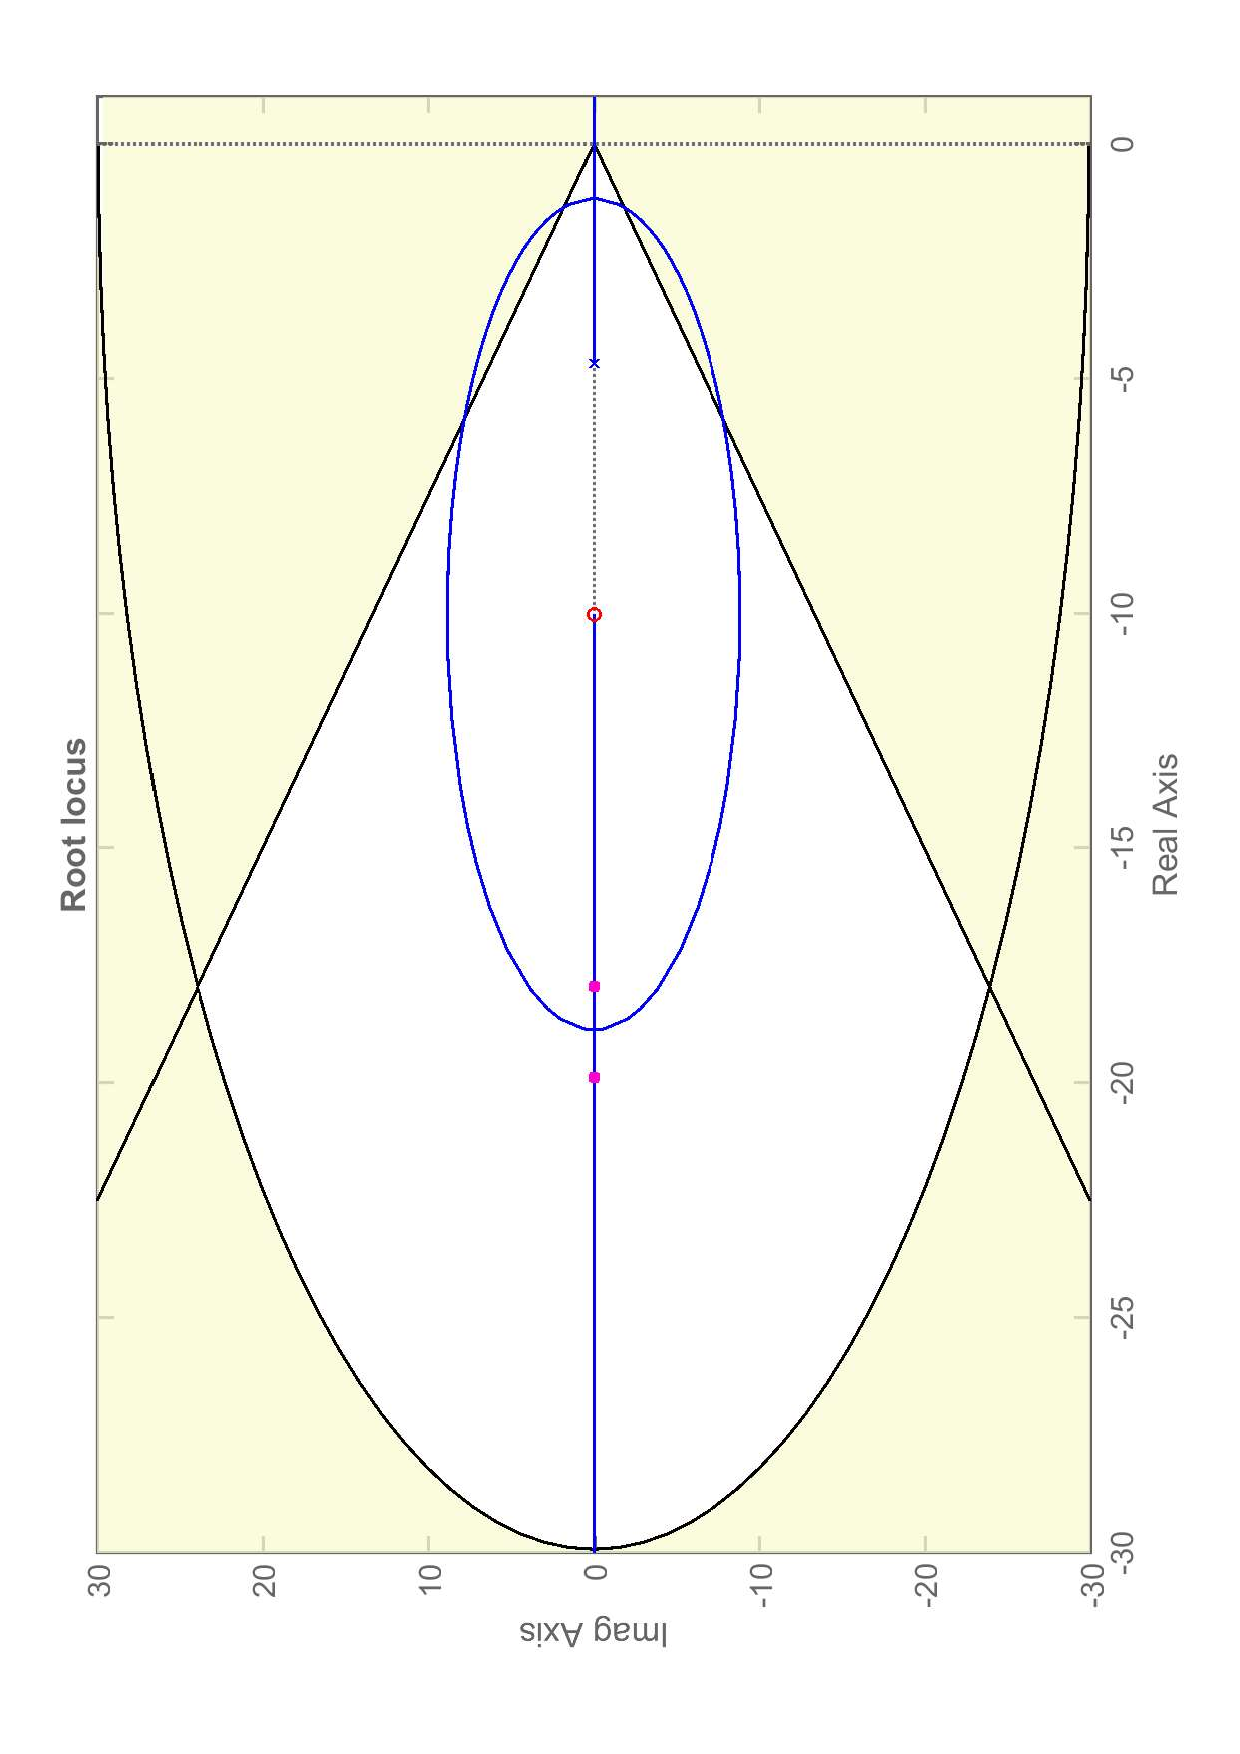
\includegraphics[height=0.75\textwidth,angle = -90]{figures/locusReq.pdf}
\caption{The root locus diagram of the open loop, with the requirement for damping and natural frequency included. The white area is the area where the requirements are met.}
\label{fig:locus2}
\end{figure}
\vspace{-0.5 cm}
The controller can thus be written as:
\begin{equation}
D(s) = \frac{(s + 10)160}{s}
\end{equation}
The bode plots for the open loop of the outer loop is shown in \autoref{fig:bodeInvPen}.
\begin{figure}[H]
\centering
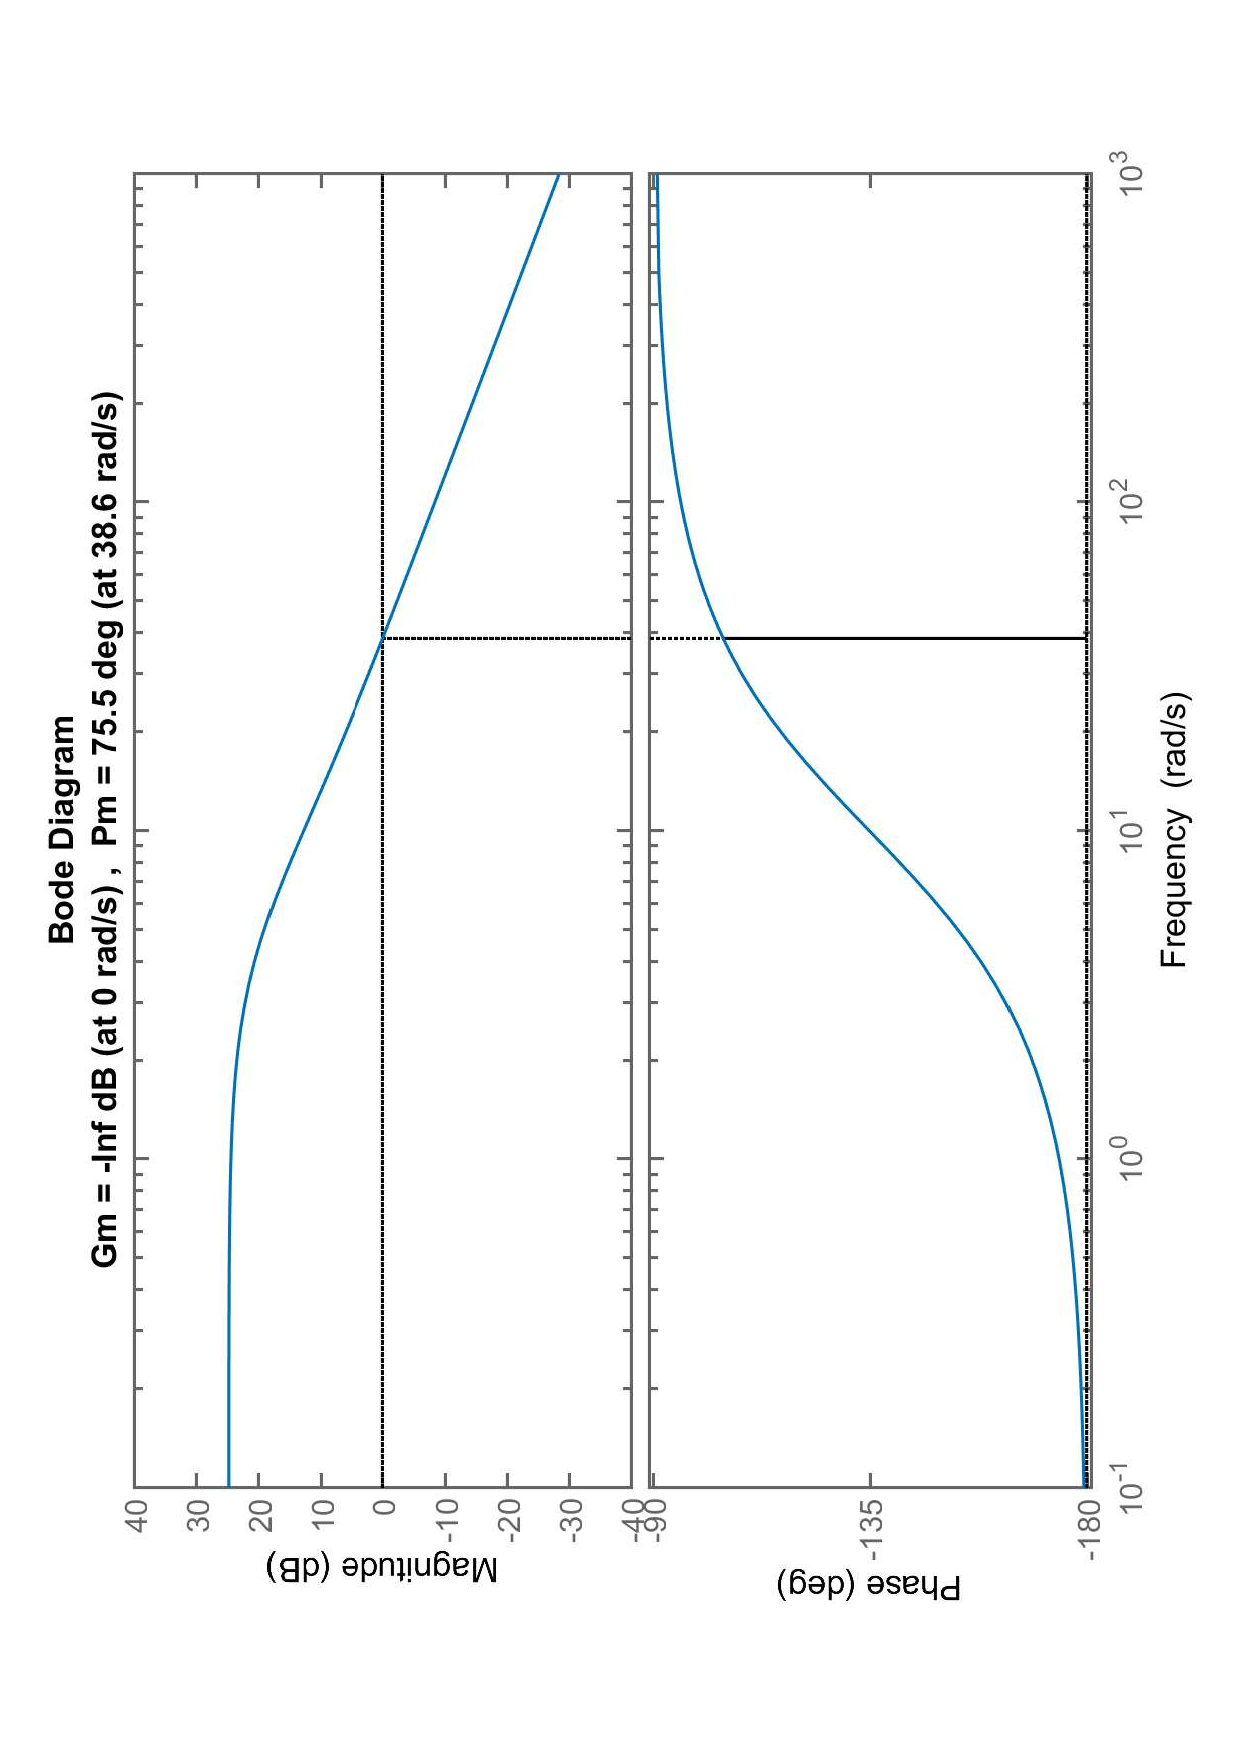
\includegraphics[height = 0.85\textwidth, angle = -90]{bodeOuterLoop.pdf}
\vspace{-0.7 cm}
\caption{The open loop bode plots of the outer loop.}
\label{fig:bodeInvPen}
\end{figure}
From this it is seen that the phase margin and gain margin requirements are not met. This is not an issue, as the system has been stabilized as a closed loop system, due to the root locus method. Thus the behaviour of the open loop system is not required to be stable. Since the phase and gain margins are stability criterias for the open loop, which is not required to be stable, the issue is disregarded.
A simulation of the step response of the outer loop, with this controller is shown in \autoref{fig:stepInvPen}.
\begin{figure}[H]
\centering
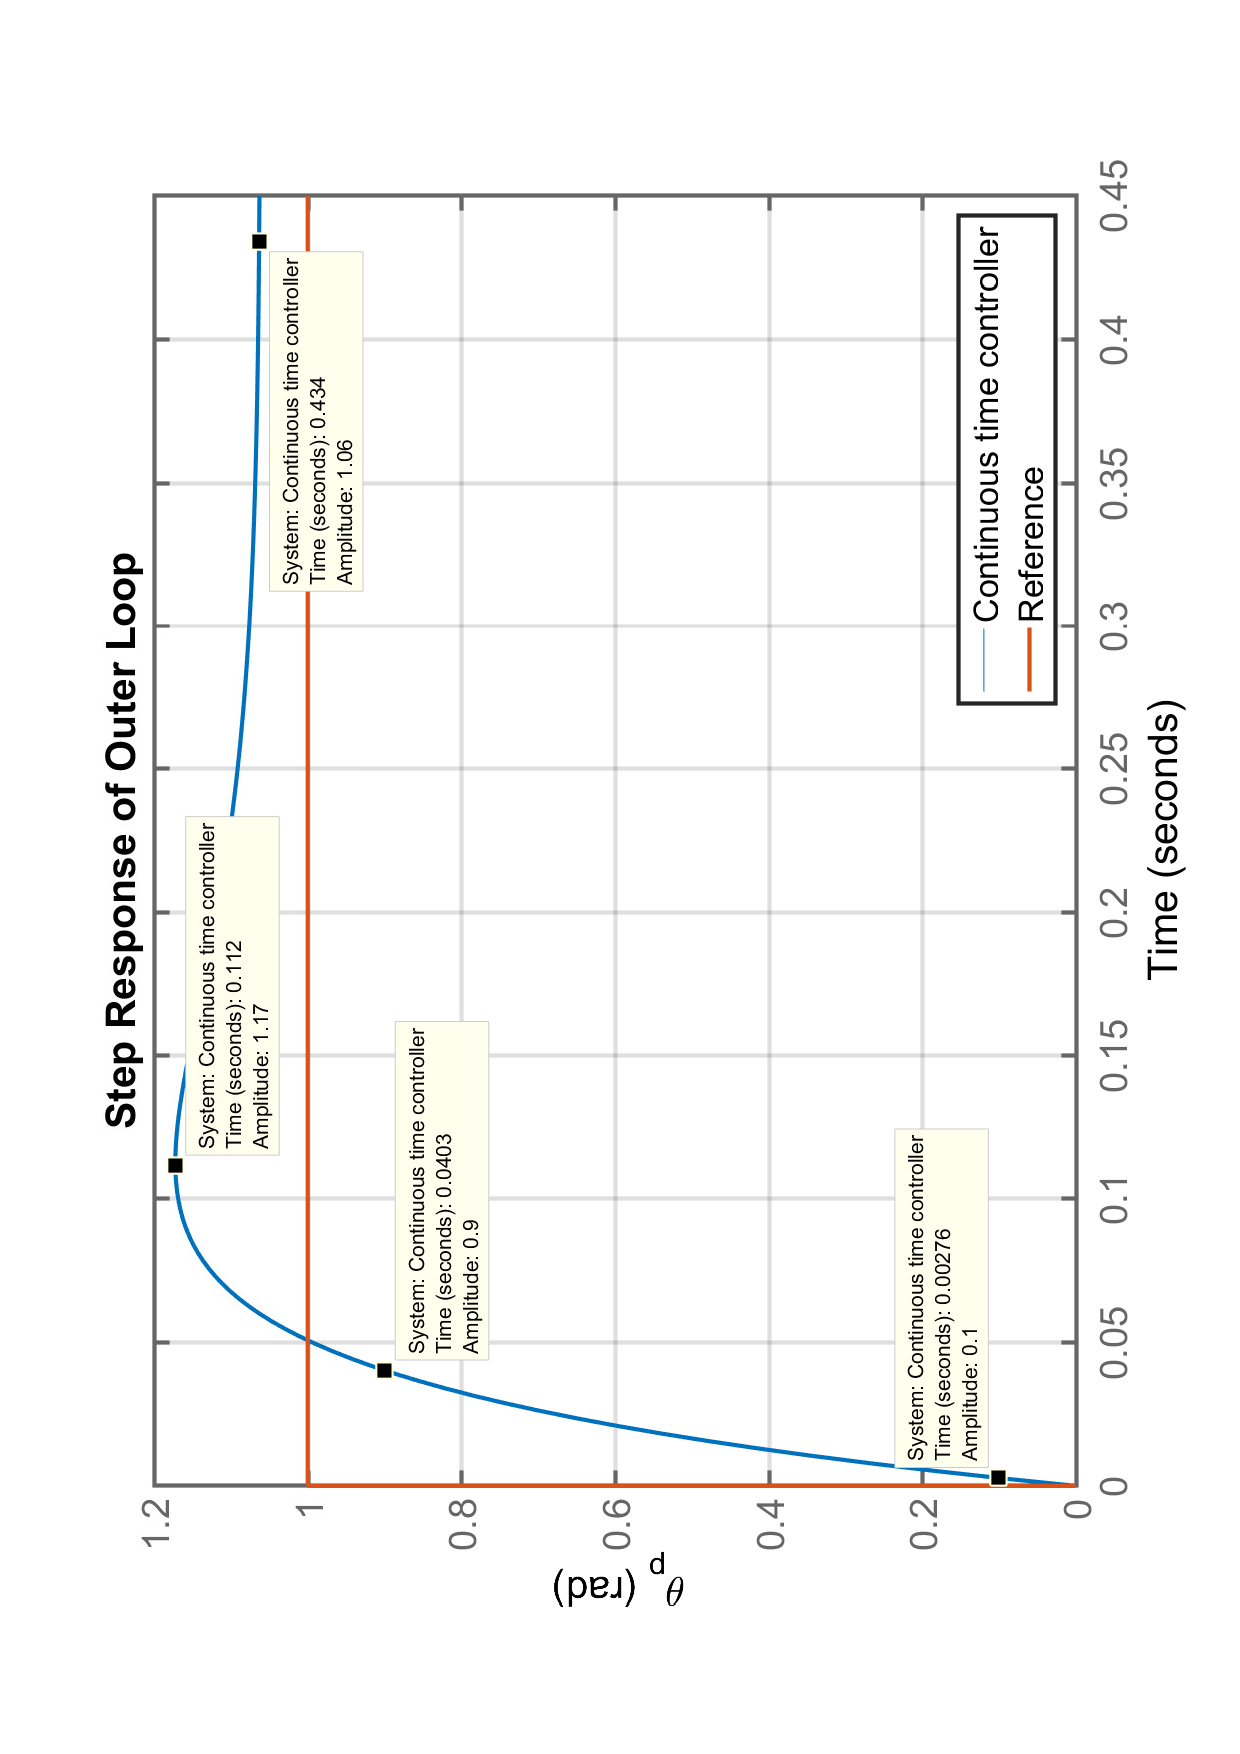
\includegraphics[height=\textwidth,angle = -90]{figures/invPenStep.pdf}
\caption{Simulation of the step response of the outer loop with the designed continuous time PID-controller.}
\label{fig:stepInvPen}
\end{figure}

From the step response, the following dynamics are determined as:
\begin{itemize}
\item Rise time: $t_r = 0.038 s$
\item Steady-state error: $e_{ss} = 6$ \%
\item Overshoot: MP = 9.4 \%
\item The system never settles at 1 in amplitude, it does however reach a steady state at approximately 0.45 s. Thus $t_s \approx 0.45 s$.
\end{itemize} 

Comparing these system dynamics with the requirements, it is seen that the rise time, settling time and overshoot are within the requirements. On the other hand, a steady-state error is present which is a violation of the requirements. The reason for the steady-state error is that the closed loop is of system type zero \citep[p. 211]{sou:Feedback}. This can however be corrected by an additional cascade which will not be designed or implemented due to time constraints. The system is stable and most of the requirements are met. 

%The system could be improved on with the use of compensators or an additional loop. 
%The task is to determine an appropriate $k_{p1}$. This is done through consideration of saturation. It has been tested, \autoref{app:coloumbTest}, that the maximum velocity of the segway, is $\dot x_c(t) = 1.17 \frac{\text{m}}{\text{s}}$. This leads to $\omega_w(t)$ saturating at: $\omega_w(t) = \frac{\dot x_c(t)}{r_w} = 10 \frac{rad}{s}$. To avoid sudden saturation it is decided to design the controller, so that error signals of up to 2 rad/s does not cause saturation, assuming a start velocity of zero. \\
%To determine the $k_p$ factor from this, the controller is inverse laplace transformed, yielding:
%\begin{equation}
%d_1(t) = k_{p1} \cdot \delta(t) + k_{p1} \cdot k_z = k_{p1} \cdot \delta(t) + k_{p1} \cdot 10
%\end{equation}
%The output of the controller, $\omega_w(t)$, is expressed as:
%\begin{equation}
%\omega_w(t) = e(t) \cdot k_{p1} \cdot \delta(t) + k_{p1} \cdot k_z \cdot \int e(t) dt
%\end{equation}
%\begin{where}
%\va{$e(t)$}{is the error signal}{1}\\
%\va{$\delta(t)$}{is the delta function}{1}\\
%\end{where}
%
%Based on the previous considerations, $k_{p1}$ can be determined as shown in \autoref{eq:k_pCal}, where the last term is zero, as only a momentary change is considered. Thus the integral term is zero. The delta function, $\delta(t)$, is equal to $1$ as the controller is a discrete system.
%\begin{equation}
%k_{p1} = \frac{\omega_w(t)}{e(t)} = \frac{10}{2} = 5\label{eq:k_pCal}
%\end{equation}
%The closed loop pole locations are now determined through analysis of the basic feedback system's closed loop:
%\begin{equation}
%\frac{Y_1(s)}{R_1(s)} = \frac{D_1(s) \cdot G_1(s)}{1 + D_1(s) \cdot G_1(s) \cdot H_1(s)}
%\end{equation}
%\begin{where}
%\va{$Y_1(s)$}{is the output of the outer controller}{1}\\
%\va{$R_1(s)$}{is the input of the outer controller}{1}\\
%\va{$H_1(s)$}{is the sensor block of the outer controller}{1}\\
%\end{where}
%In the following the enumerator is ignored as the focus is on the closed loop poles, which is the solution to the characteristic equation:
%\begin{equation}
%1 + D_1(s) \cdot G_1(s) \cdot H_1(s) = 0
%\end{equation}
%Since H(s) for the segway is a constant factor of 1, the characteristic equation can be written as it is in \autoref{eq:chaEQ2}, where the plant and controller transfer functions have been inserted.
%\begin{equation}
%1 + \frac{(s + 10)5}{s} \cdot \frac{0.2367 \cdot s}{s^2 - 21.92} = 0\label{eq:chaEQ2}
%\end{equation}
%Rearranging \autoref{eq:chaEQ2} yields:
%\begin{equation}
%s^2 - 21.92 + (s + 10)1.184 = s^2 + 1.184 \cdot s + 25.44 = 0
%\end{equation}
%The location of the closed loop poles are found through solving this quadratic equation. This yields a pole in $-0.592 - 5.01i$ and the other pole is the complex conjugate of this pole. Both poles are in the LHP, thus the controller:
%\begin{equation}
%D_1(s) = \frac{(s + 10)5}{s}
%\end{equation}
%Assures that the closed loop poles are in the LHP, yielding a stable system.
%
%Before implementing this controller on the microcontroller, it has to be discretized. The discretization is performed with the bilinear transform shown
%\todo{Write the discretization part.}
%
%
%
%In the following, a method of assuring pure LHP poles for this plant is derived. This is done with outset in the basic feedback systems closed loop:
%
%\begin{equation}
%\frac{Y(s)}{R(s)} = \frac{D(s) \cdot G(s)}{1 + D(s) \cdot G(s) \cdot H(s)}
%\end{equation}
%
%The enumerator will be ignored for now as the focus is on the closed loop poles, which is the solution to the characteristic equation:
%
%\begin{equation}
%1 + D(s) \cdot G(s) \cdot H(s) = 0
%\end{equation}
%
%Since H(s) for the segway is a constant factor of 1, the characteristic equation can be written as it is in \autoref{eq:chaEQ2}, where the plant equation has also been inserted.
%
%\begin{equation}
%s^2 - 15.47 + D(s) \cdot 0.04609 \cdot s\label{eq:chaEQ2}
%\end{equation}
%
%
%
%
%
%
%
%
%
%
%
%
%
%
%
%
%
%
%unstable - make it stable\\
%move zero to LHP\\
%PD controller as result\\

Now the controller can be discretized. This is done in MATLAB using bilinear transformation, which yields:
\begin{equation}
D_1(z) = \frac{172 z - 148}{z - 1}
\label{origControllerDiscrete}
\end{equation}

This controller is compared to the continuous time controller which can be seen in \autoref{fig:sysStep2}. 

\begin{figure}[H]
\centering
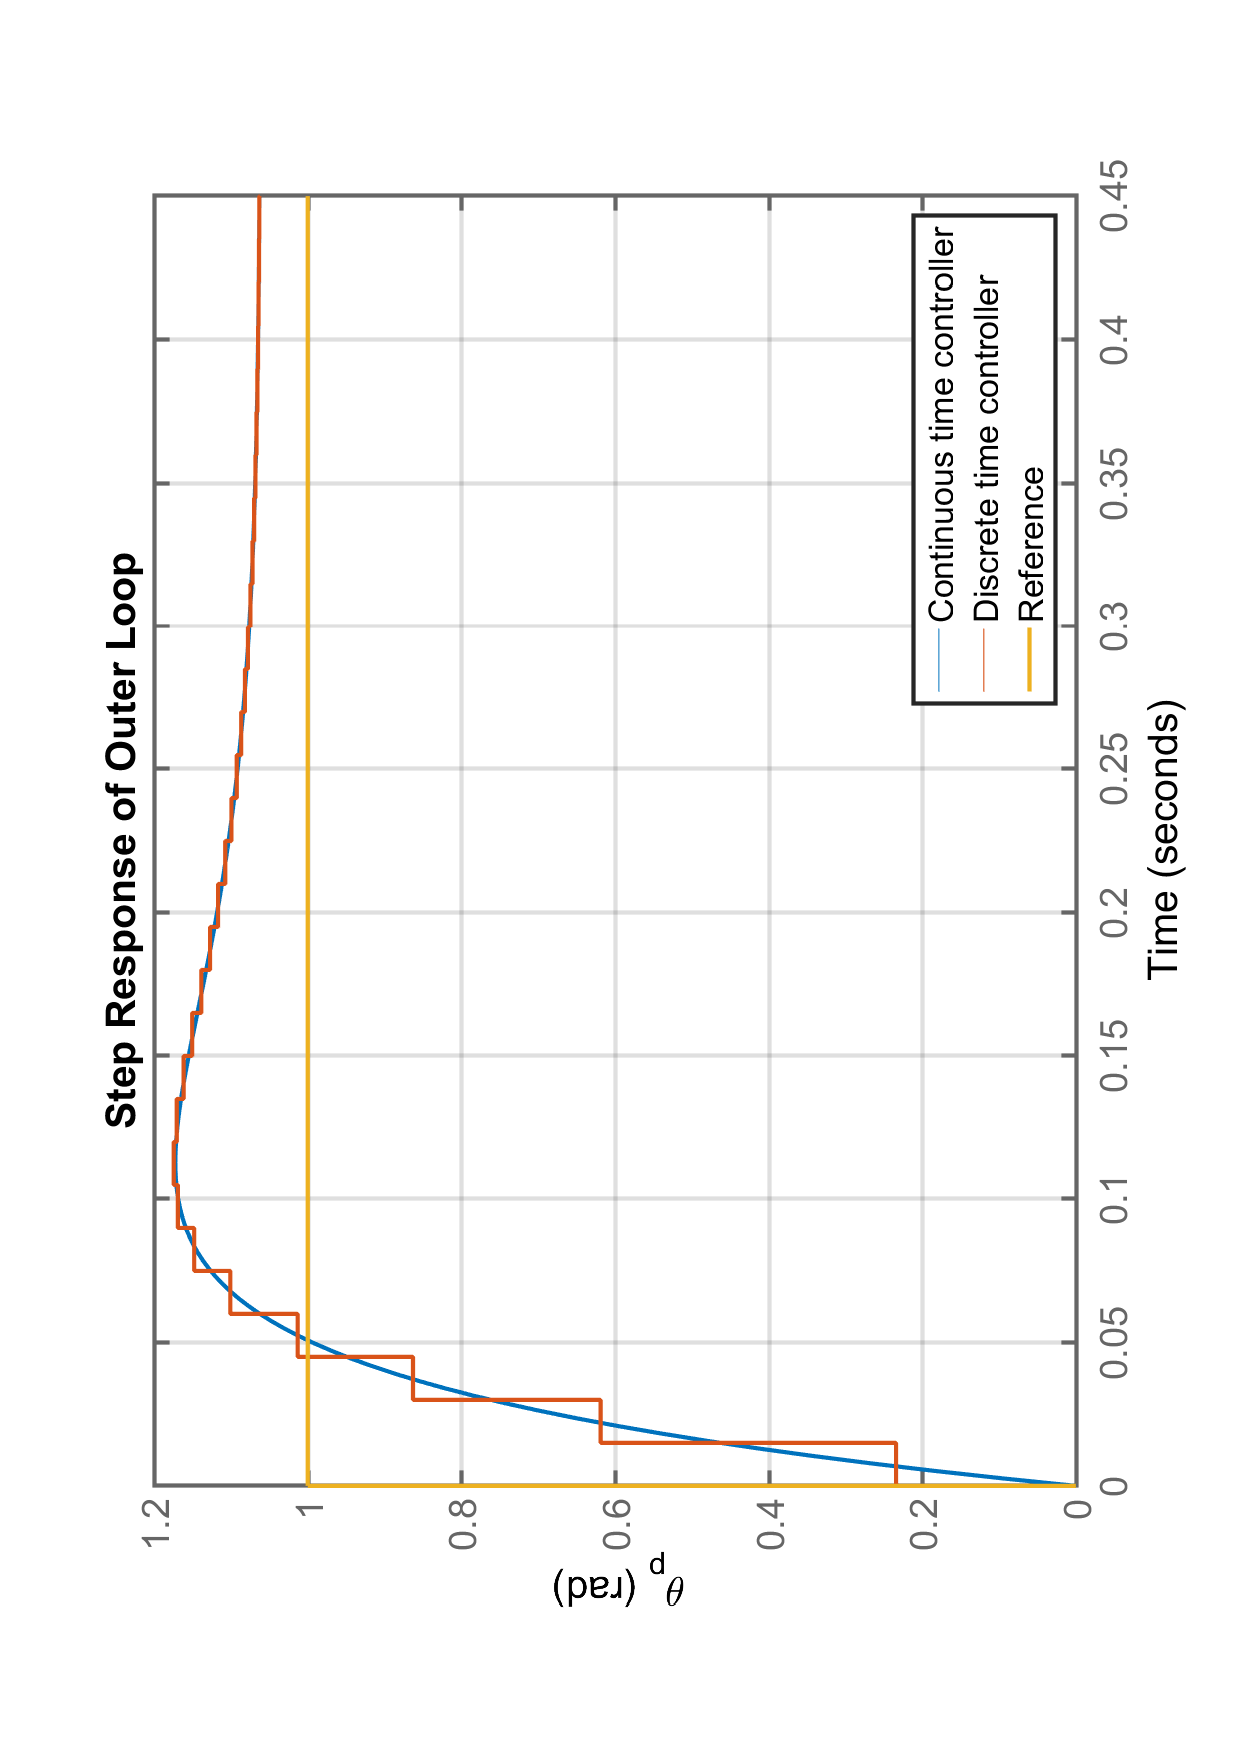
\includegraphics[height =\textwidth ,angle = -90]{sysStep2.pdf}
\caption{Simulation of the step response of continuous and discrete outer loop controller.}
\label{fig:sysStep2}
\end{figure}

From \autoref{fig:sysStep2} it can be seen that the discrete controller matches the continuous controller. The controller design is therefore satisfying.

\section{Validation of Cascade Controller}
The final step before implementing the controller is to verify that it can stabilize the model as well as the linearised model. For this purpose the controllers have been implemented in MATLAB. Note that the inner loop controller has been implemented as a continuous time controller due to simplicity, and a step on the reference is applied. This step is set to 0.1 radians instead of 1 radian as the controller is designed to work close to the operating point and 1 radian is seen as too far away. Due to the characteristics of the linearity of the linear model it is still possible to compare the results from this simulation to the simulation of the linear control system. The result can be seen in \autoref{fig:controllerVerification}. 
\vspace{-0.75 cm}
\begin{figure}[H]
\centering
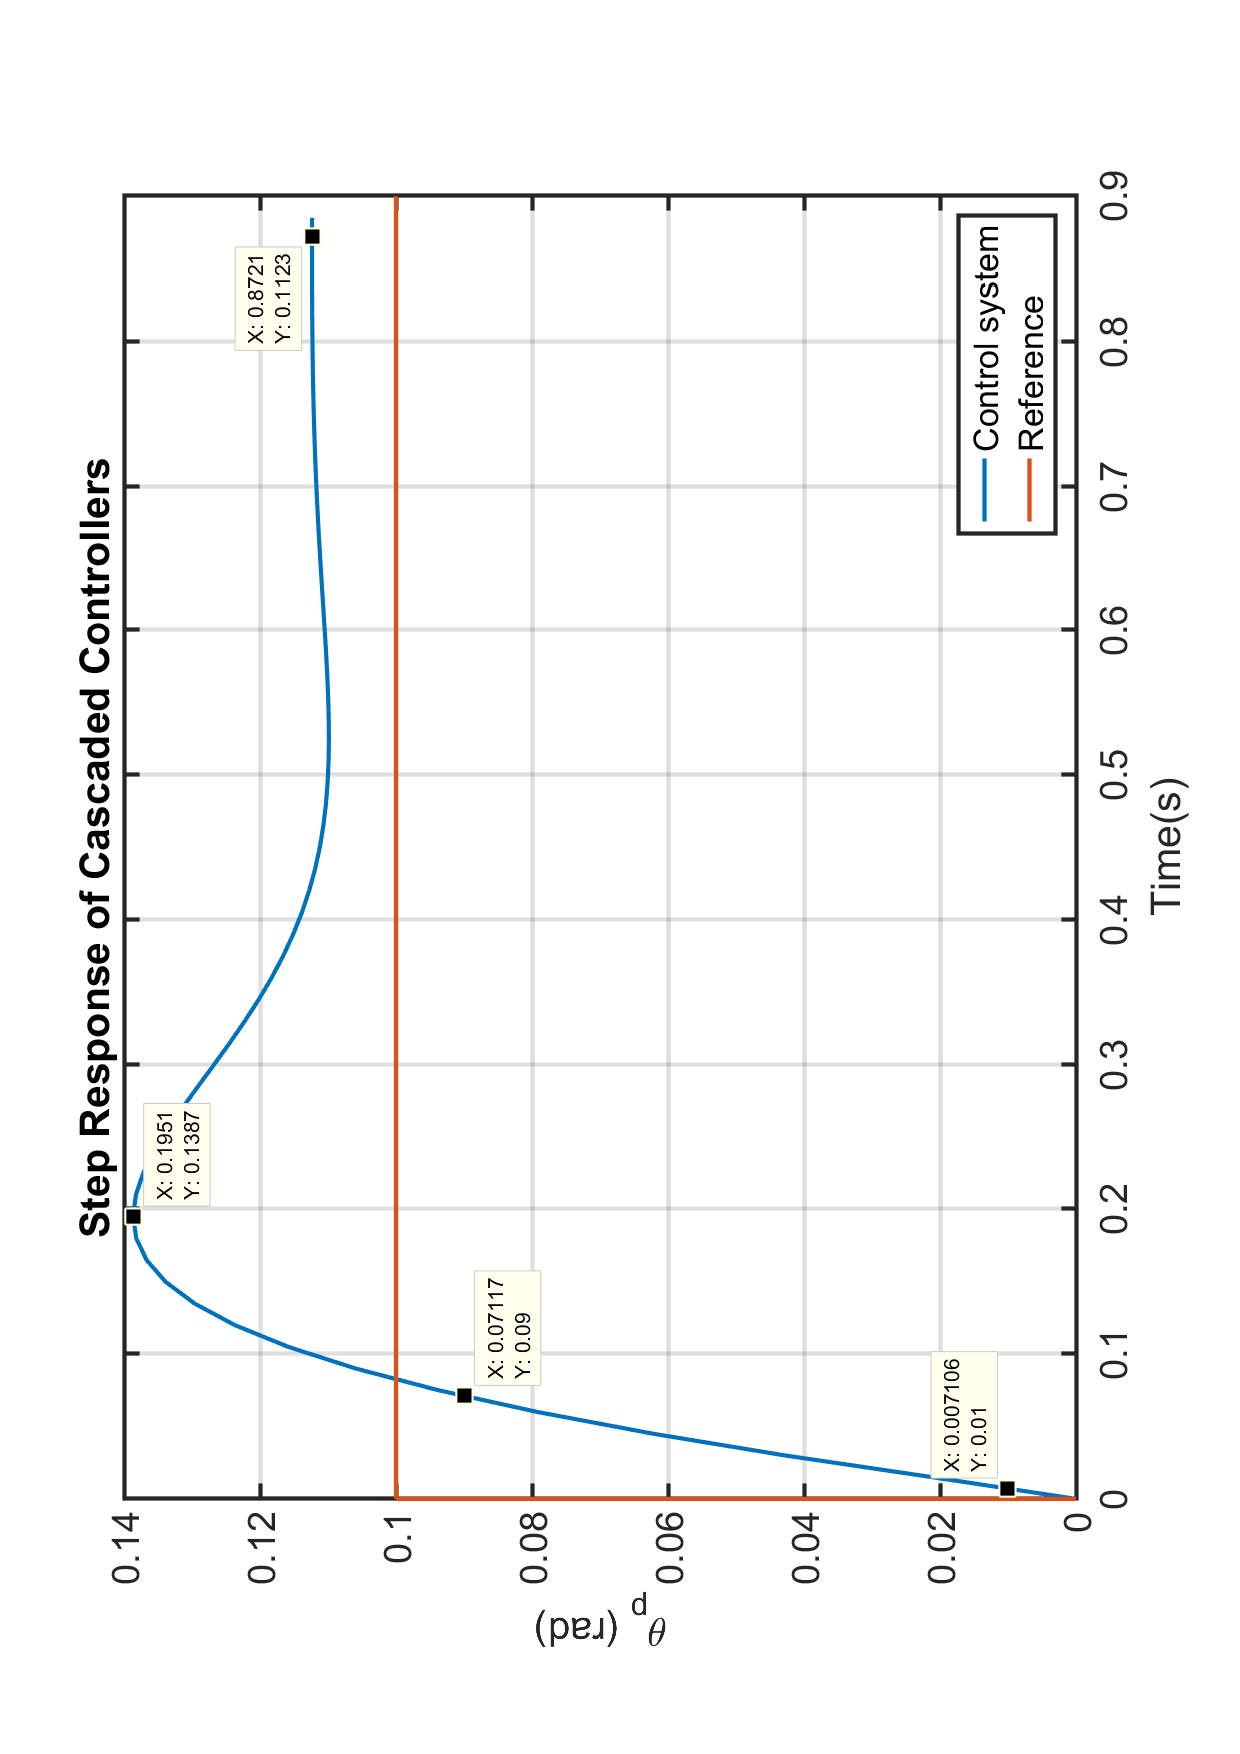
\includegraphics[height =\textwidth ,angle = -90]{controllerVerification.pdf}
\caption{Simulation of the step response of the control system consisting of a discrete outer loop controller a continuous inner loop controller and the original model.}
\label{fig:controllerVerification}
\end{figure}
From the step response seen in \autoref{fig:controllerVerification}, the following dynamics are determined:
\begin{itemize}
\item Rise time: $t_r = 0.064 s$
\item Steady-state error: $e_{ss} = 12.3$ \%
\item Overshoot: MP = 23.5 \%
\item The system never settles at 1 in amplitude, it does however reach a steady state at approximately 0.7 s. Thus $t_s \approx 0.7 s$.
\end{itemize} 

From this it can be seen that two of the requirements are met and two are not met, where, for the linearised model, only the requirement for the steady-state error were not met. This may be due to differences between the linearised model and the model. Since these differences most likely arise from the problems mentioned in parameter estimation of the inverted pendulum model, this is not considered an issue as it is assumed that tuning can correct this.

% however this is not considered an issue since the possibility of tuning correcting this still exist.

\section{Implementation of Cascade Controller}
After implementation of the controllers on the segway, it is seen that the segway overreacts to errors. Therefore the controller coefficients for the outer loop controller are adjusted, resulting in the following final implementation:
\begin{equation}
D(z)=\frac{3.8-2.56\cdot z^{-1}}{1-z^{-1}}
\end{equation}

The reason for the substantial adjustment compared to the original implementation in \autoref{origControllerDiscrete}, might be due to either that the model is missing something critical or that the effects of the saturation is not negligible as anticipated. If this controller is applied to the linear model, the simulation of a step on the reference results in an unstable response, which is not surprising since the adjustment is quite substantial. This could show that the model does not describe reality as well as expected, possibly due to a sign error or an implementation error in the model. This will however not be further investigated due to time constraints.
%\begin{figure}[H]
%\centering
%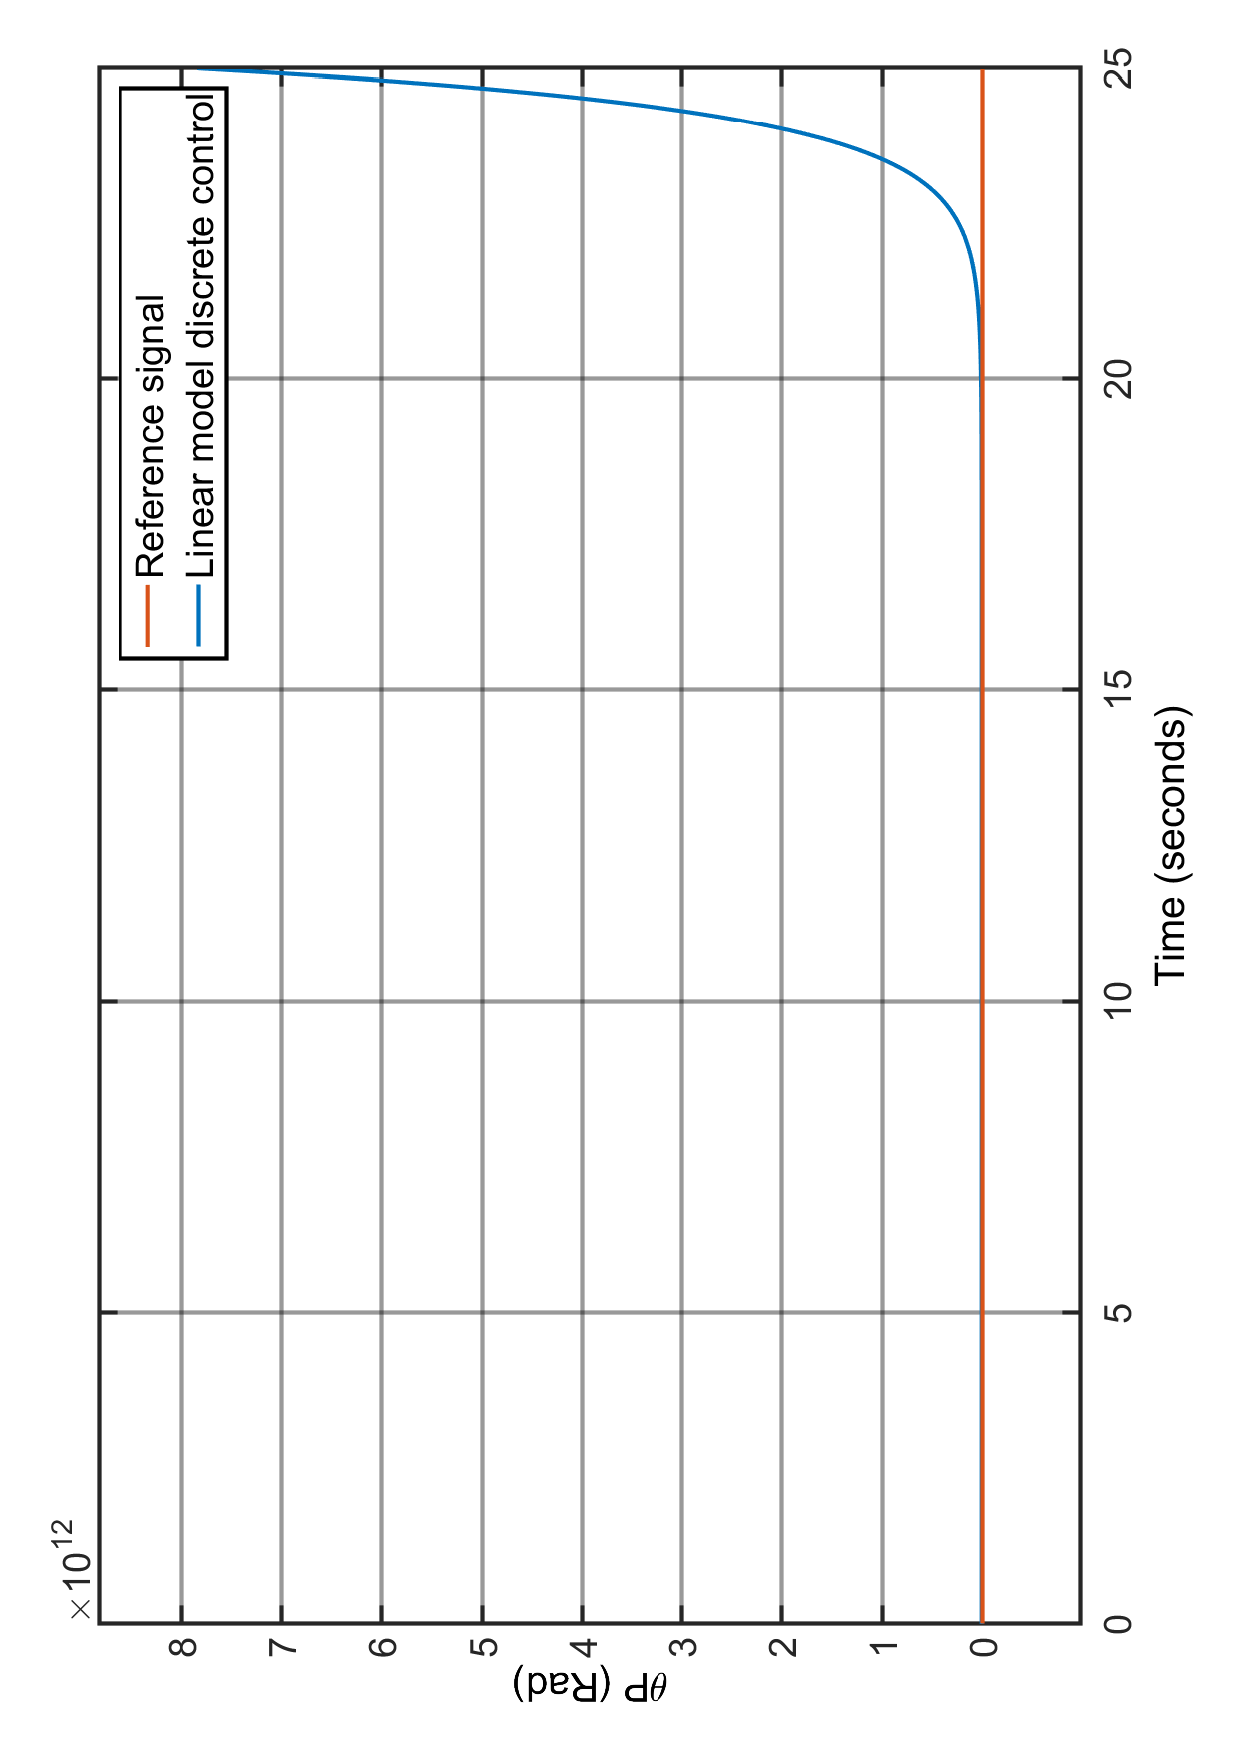
\includegraphics[height = \textwidth, angle = -90]{stepControlSys4.pdf}
%\caption{Simulation of implemented controller on linear model.}
%\label{fig:stepControlSys4}
%\end{figure}

With the implemented controller, the system has become stable. Filters can now be designed to reduce sensor noise.
